\subsubsection*{Le matin :}
Voici le graphique attendu :
\begin{figure}[H]
    \center
    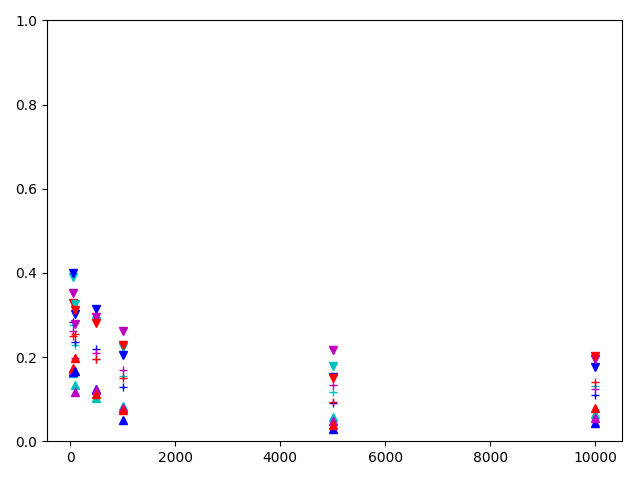
\includegraphics[height=\grand]{sources/data/etfdata/graph2}
	\caption{Ecart type de l'apprentissage en fonction de la taille de la base de données}
	\label{etfdata2}
\end{figure}

Ici, contrairement à la Fig.\ref{etfdata1}, une décroissance est visible.

\subsubsection*{L'après midi :}
Le reste de la journée à été passée a générer des données.
Le programme à été legerement modifié:
Au lieu de creer un graphique directement, les données sont stoquées en \textsc{JSON}.
On peut ensuite creer un graphique à partir de ces données.
